\documentclass[12pt]{article}
\usepackage[utf8]{inputenc}
\usepackage{amsmath}
\usepackage{amsfonts}
\usepackage{amssymb}
\usepackage{multicol}
\usepackage{booktabs}
\usepackage{graphicx}
\usepackage{array}
\usepackage{multicol}
\usepackage{indentfirst}
\usepackage{longtable}
\usepackage{threeparttable}
\usepackage{setspace}
\usepackage{cite}
\usepackage[numbers,sort]{natbib}
\usepackage{titlesec}
\usepackage{titletoc}
\usepackage[titletoc]{appendix}
\usepackage{nameref}
\usepackage{fontspec}
\setmainfont{Times New Roman}
\pagestyle{plain}
\linespread{1.6}
\setlength{\parindent}{2em}

\begin{document}

\begin{center}
    \vspace{-1cm}
    
\includegraphics[width=0.43\paperwidth]{zju.pdf}
    \\
    \Large{Fixed Income Analytics and Models: Group Project\\}
    \vspace{0.6cm}
    \emph{\Large Team Members\\}
    \large 
    \setlength{\tabcolsep}{3mm}{
    \begin{tabular}{lll}
        \vspace{-0.2cm}
        Zhang Mingyue & 3200105091 & 3200105091@zju.edu.cn\\
        \vspace{-0.2cm}
        Yao Zongqing & 3200103341 & 3200103341@zju.edu.cn\\
        \vspace{-0.2cm}
        He Rouhan & 3200103563 & 3200103563@zju.edu.cn\\
        \vspace{-0.2cm}
        Qu Mingqi & 3200105083 & 3200105083@zju.edu.cn\\
        \vspace{-0.2cm}
        Zhang Yanhui & 3200103609 & 3200103609@zju.edu.cn\\
        \vspace{-0.2cm}
        Huang Niyuan & 3200101028 & 3200101028@zju.edu.cn\\
        \vspace{-0.2cm}
        Chen Yirui & 3200104816 & 3200104816@zju.edu.cn\\
        \vspace{-0.2cm}
        Li Xinyi & 3200104813 & 3200104813@zju.edu.cn\\
    \end{tabular}
    }
\end{center}

\newpage

\tableofcontents

\newpage

\section{Introduction}
\indent In this paper we use time-series data to forecast government bond excess yields in the United States. Our work extends Ludvigson and Ng (2009)\cite{ludvigson2009macro} classic regressions. We selected forward rates, macroeconomic fundamentals and added factors of investors' subjective beliefs and the supply of government debt to run the regression. 

Reviewing the past literature, we analyze a variety of factors that have predictive power for bond excess returns in a comprehensive analysis. We selected the nine most representative macro variables, introduced two other dimensional explanatory variables, conducted regression tests using the data, and found that these factors significantly affect the in-sample excess return fit. However, after dividing the sample into in-sample and out-of-sample data, it was found that the out-of-sample predictions were not good. We then used a machine learning algorithm to obtain a model that could predict excess returns better by adjusting the parameters and constructed a simple strategy that, after back-testing, achieved positive excess returns.

\section{Literature Review}
\indent Fama and Bliss(1987)\cite{fama1987information} shows that the excess return of U.S. Treasury could be predicted by both forward and spot interest rates. Furthermore, when the forecast horizon is extended,the forecast power of forward rates improves, which reflects a slow mean-reverting tendency of interest rates.
$$
r(x-1:t+1)-r(x-1:t)=-a_2+(1-b_2)[f(x,x-1:t)-r(1:t)]-u_2(t+1)
$$

On the basis of Fama and Bliss's paper, Cochrane and Piazzesi (2005)\cite{cochrane2005bond} studied time variation in expected excess bond returns and ran regressions of one-year excess returns on initial forward rates. Moreover,they found that a single factor, viz. a single tent-shaped linear combination of forward rates predicts excess returns on one- to five-year maturity bonds with a 0.44 $R^2$
$$
rx^{(n)}_{t+1}=\beta^{(n)}_{0}+\beta^{(n)}_{1}y^{(1)}_{t}+\beta^{(n)}_{2}f^{(2)}_{t}+\ldots+\beta^{(n)}_{5}f^{(5)}_{t}+\varepsilon^{(n)}_{t+1}
$$

After that, scholars tried to bypass the bond market data and forecast it from a macroeconomic perspective. Ludvigson and Ng (2009)\cite{ludvigson2009macro} revealed that there is a possible empirical linkages between predictable variation in excess U.S. government bonds and macroeconomic fundamentals by using the methodology of dynamic factor analysis for large datasets.They found that strong predictable variation in excess bond returns associates with macroeconomic activity and traditional pure financial variables omit pertinent information connected with macroeconomic fundamentals.Also,it stressed that it is important to use information beyond that contained in the yield curve for uncovering countercyclical, business cycle-frequency variation in bond risk premia.
$$
rx^{(n)}_{t+1}=\beta_{0}+\beta^{'}_{1}\widehat{F_{t}}+\beta_{2}CP_{t}+\varepsilon_{t+1}
$$

In addition to the above directions, Laborda and Olmo (2014)\cite{laborda2014investor} incorporate a sentiment factor to document a positive relationship between investor sentiment and expected excess bond returns. Specifically,when the economy is in turmoil and investor sentiment is depressed,this mechanism operates through the choice of bonds.And when investor sentiment is high,this mechanism, in turn, works through stocks.Moreover,investor sentiment is a mirror of future interest rate dynamics and monetary policy. Sluggish market sentiment means higher interest rates in the future.

Finally, we also found some special perspectives. Bond Supply and Excess Bond Returns\cite{greenwood2014bond} proved that the supply and maturity structure of government debt are positively correlated with bond yields and expected returns. Additionally,holding the short rate constant,these effects should be stronger for longer-maturity bonds and during times when arbitrageurs are more risk-averse.

\section{Theoretical Framework}
\subsection{Model Theory}
\indent Our theory mainly builds on the model of Ludvigson and Ng (2009)\cite{ludvigson2009macro} and Cochrane and Piazzesi (2005)\cite{cochrane2005bond}.  Variables on the supply of government debt and investor sentiment to optimize were added according to our empirical principles of economics to improve the classical model's predictive ability.

A linear combination of five forward spreads explains excess returns in the next year in bond with maturity raging from 2 to 5 years. Treasury yields can be decomposed into inflation expectations and term-specific interest rate cycles. According to Fisher equation, the nominal short-term interest rate is the sum of a range of expected inflation rates and short-term real interest rates. We noticed that the expected inflation rate is in continuous change, usually called the trend inflation rate, which together with the term determines the level of long-term interest rates. Reflecting the trend inflation rate in terms of past real core inflation rates reflects people's slowly changing inflation rate expectations over time.For another part-term-specific interest rate cycles, Cochrane and Piazzesi (2005)\cite{cochrane2005bond} define variable cycle as the change in the rate of return orthogonal to the expected inflation rate

Therefore, we believe that the linear combination of forward rates can predict the future inflation rate well.

However, some studies indicate that the predictive power of CP variable has declined in recent years. When we expand our data to 1964.1 to 2003.12, the regression shows that the adjusted $R^2$ statistic decreased significantly from $R^2$ = 0.44 in Cochrane and Piazzesi (2005)\cite{cochrane2005bond} to $R^2$ = 0.34 in Ludvigson and Ng (2009)\cite{ludvigson2009macro}. Therefore, considering that the bond market data cannot fully reflect the market changes, we add some macroeconomic fundamentals to improve the forecasting power for excess bond returns.

We analyse on the basis of the 132 macro fundamental variables mentioned in paper of Ludvigson and Ng (2009)\cite{ludvigson2009macro}. According to the multicollinearity between variables and the degree of influence on bond prices, we screen out 9 variables that we believe to be potentially influential factors. Based on Ludvigson and Ng(2009)\cite{ludvigson2009macro}, the variables of personal income(PI), help-wanted advertising(Hw), civilian labor force(Cps), employees on nonfarm payrolls(Emp), average working hours(Avghrs), housing starts(Starts), installment credit/PI ratio(Inst) are selected to measure the real factor, concerning employment and production, which has been confirmed the most important factor in regression of Ludvigson and Ng (2009)\cite{ludvigson2009macro}. These variables are low in recessions and high in booms, capturing marked cyclical variation in real activity. Connecting these variables to the forecasts of excess bond returns, we finally find the negative correlation between them, which is consistent with economic theories that investors must be compensated for bearing risks related to recessions. In addition, we choose the variable of exchange rate(Ex rate) to reflect the level of interest rates and CPI as the inflation factor. Indeed, these factors contain economically meaningful information that is not contained in CP enhancing the predictive power of our model.

We also consider the role of sentiment factor and the bond supply with statistical power to explain variation on the bond risk premia.

Our regression eventually documents a negative relationship between investor sentiment variables and expected excess bond returns that is above and beyond the information contained in the term structure of bonds and macroeconomic factors. The finding suggests that bonds can appear overpriced when market sentiment is high because of the excessive demand, which depresses its ex post return. On the contrary, low market sentiment may lead to higher excess returns on bonds.

\centerline{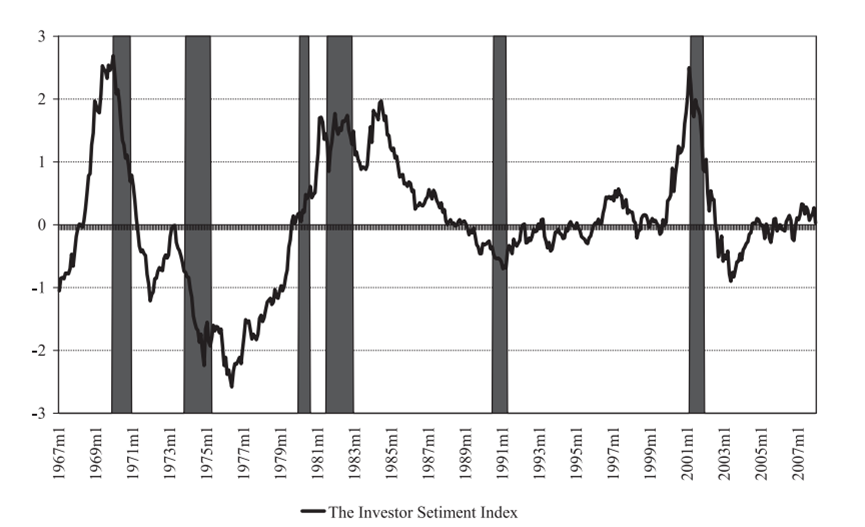
\includegraphics[scale=0.47]{Figure1.png}}

An increase in supply should raise bond yields and expected returns, holding the short rate constant. Changes in supply in our model affect the duration risk that arbitrageurs need to bear, since arbitrageurs are the only subject absorbing shocks . When the supply of long-term bonds increases, arbitrageurs have to absorb more bonds to accommodate the increased supply, who require higher expected returns in excess of the short rate to compensate for their higher duration. Consequently, bond prices go down, and excess yields go up. 

Explanation above makes sense since the yields are higher and prices are lower for the increasing supply of longer-maturity bonds.

\subsection{Data and Variable Selection}
We test the predictions of our model using data on the U.S. Treasury market from 1964.1 to 2003.12. We conduct monthly observations on the excess yields of bonds maturing in 2, 3, 4, and 5 years.

Ludvigson and Ng(2009)\cite{ludvigson2009macro} obtained 8 factors by principal component analysis method for 132 macro variables, and these factors and function forms can be used to carry out regression analysis on the bond excess return rate. However, we note that the 132 macro variables are highly homogeneous and partially correlated. Based on economic theory and considering the multi-collinearity among the variables, we selected 9 most representative macro variables, and introduced another 2 other explanatory variables (see Table 1 for the definition of specific variables). 

We also control the linear combination of forward interest rates from the dataset of Cochrane and Piazza Si (2005)\cite{cochrane2005bond}.

With reference to Baker and Wurgler(2006)\cite{baker2006investor}, we define the investor sentiment index as the first principal component of the correlation matrix of five variables underlying proxies for sentiment.\footnote{These proxies, orthogonalized to several macroeconomic variables, are: (1) the closed-end fund discount;  (2) the number of IPOs; (3) the average first-day returns; (4) the share of equity issues in total equity and debt issues; (5) the dividend premium.} For the supply of bonds, we scale it by GDP, and term it the maturity-weighted-debt-to-GDP(Mwd), which is approximately the product of debt to GDP times the average maturity of debt.

\section{Data and Methodology}
\subsection{Definitions of Variables}
\begin{table*}[ht!]
    \centering
    \caption{Definitions of Main Variables}
    \setlength{\tabcolsep}{9mm}{
    \begin{tabular}{|l|l|}
        \hline
        PI & Personal income\\
        \hline
        Hw & Index of help-wanted advertising\\
        \hline
        Cps total & Civilian labor force: total\\
        \hline
        Emp & Employees on nonfarm pay rolls\\
        \hline
        Avg hrs & Average working hours\\
        \hline
        Starts & Housing starts\\
        \hline
        Inst & Ratio: Installment credit/PI\\
        \hline
        Ex rate & Exchange rate\\
        \hline
        CPI & CPI\\
        \hline
        Sent & Investors sentiment\\
        \hline
        Mwd & the maturity-weighted-debt-to-GDP ratio\\
        \hline
        CP & Cochrane and Piazzesi(2005)\cite{cochrane2005bond} factor\\
        \hline
    \end{tabular}
    }
\end{table*}

\newpage

\subsection{Basic Data Parameters}

\begin{table*}[htp!]
    \centering
    \caption{Summary Statistics}
    \setlength{\tabcolsep}{9mm}{
    \begin{tabular}{cccc}
        \toprule
        Variables & (1) & (2) &(3) \\
         & Mean & Min & Max \\ 
        \midrule
        PI & 66671.409 & 2562.5 & 11595.7\\
        Hw & 79.963 & 63.82 & 91.64\\
        Cps total & 77.302 & 40 & 115.13\\
        Emp & 657.978 & 498 & 1177.4\\
        Avg hrs & 40.158 & 37.2 & 41.3\\
        Starts & 1485.403 & 478 & 2494\\
        Inst & 2.243 & -41 & 62.3\\
        Ex rate & 96.125 & 76.01 & 132.56\\
        CPI & 63.813 & 18 & 97.6\\
        Sent & -0.002 & -2.19 & 3.21\\
        Mwd & 2.275 & 0.671 & 4.28\\
        CP & 0.789 & -8.08 & 1.78\\
        \bottomrule
    \end{tabular}
    }
\end{table*}

\subsection{Empirical Results}
Referring to Ludvigson and Ng(2009)\cite{ludvigson2009macro}, we use the explanatory variables of one lag period to run OLS regression on the excess yields of 2-year, 3-year, 4-year and 5-year maturity bonds. In-sample regression results are shown in Table 3, in which heterogeneity robust t-statistics are reported in the parents and adjusted $R^2$ are also reported.

\newpage

\begin{table*}[htp!]
    \small
    \centering
    \caption{$rx^{(n)}=\beta_{0}+\beta_{1}X+\beta_{2}CP+\varepsilon$}
    \setlength{\tabcolsep}{6mm}{
    \begin{threeparttable} 
    \begin{tabular}{ccccc}
        \toprule
            & Panel A    & Panel B    & Panel C    & Panel D     \\
            & $rx^{(2)}$ & $rx^{(3)}$ & $rx^{(4)}$ & $rx^{(5)}$  \\
        \midrule
    PI       & -0.001***   & -0.001***   & -0.002***   & -0.002***\\
             & (-7.63)     & (-7.53)     & (-7.79)     & (-7.63)  \\
    Hw       & -0.207***   & -0.294***   & -0.390***   & -0.479***\\
             & (-6.69)     & (-4.96)     & (-4.61)     & (-4.46)  \\
    Cpstotal & -0.01       & -0.030***   & -0.038**    & -0.042*  \\
             & (-1.60)     & (-2.38)     & (-2.12)     & (-1.85)  \\
    Emp      & -0.003***   & -0.006***   & -0.008***   & -0.009***\\
             & (-5.55)     & (-5.83)     & (-5.22)     & (-4.82)  \\
    Avghrs   & -0.479**    & -1.419***   & -2.210***   & -2.637***\\
             & (-2.44)     & (-3.77)     & (-4.11)     & (-3.86)  \\
    Starts   & 0.002***    & 0.003***    & 0.006***    & 0.007*** \\
             & (-10.17)    & (-10.99)    & (-11.42)    & (-11.39) \\
    Inst     & -0.045***   & -0.080***   & -0.105***   & -0.116** \\
             & (-3.13)     & (-2.92)     & (-2.69)     & (-2.34)  \\
    Exrate   & 0.059***    & 0.107***    & 0.151***    & 0.186*** \\
             & (-6.39)     & (-6.03)     & (-5.98)     & (-5.8)   \\
    PPI      & -0.374      & 1.104       & 2.283       & 2.56     \\
             & (-0.39)     & (-0.6)      & (-0.87)     & (-0.77)  \\
    CPI      & -0.029***   & -0.058***   & -0.085***   & -0.108***\\
             & (-5.49)     & (-5.77)     & (-5.87)     & (-5.91)  \\
    Sent     & -0.391***   & -0.723***   & -1.090***   & -1.338***\\
             & (-6.85)     & (-6.61)     & (-6.99)     & (-6.76)  \\
    Mwd      & 1.090***    & 2.121***    & 3.239***    & 3.981*** \\
             & (-11.92)    & (-12.1)     & (-12.96)    & (-12.54) \\
    CP       & -0.007      & -0.134**    & -0.355***   & -0.535***\\
             & (-0.24)     & (-2.42)     & (-4.49)     & (-5.33)  \\
             &             &             &             &          \\
    Observations & 461     & 461         & 461         & 461      \\
    $R^2$-ajusted   & 0.61   & 0.57        & 0.53        & 0.5      \\
        \bottomrule
    \end{tabular}
    \begin{tablenotes} 
    \footnotesize
    \item \textit{Note:} The table reports estimates from OLS regressions of excess bonds returns on the lagged variables named in table 1. The t-statistics are reported in the parenthesis. *, **, ***represented the coefficients are statistically significant at the 10\%, 5\% and 1\% separately. A constant is always included in the regression even though its estimate is not reported in the table.
    \end{tablenotes} 
    \end{threeparttable} 
    }
\end{table*}

\newpage

The empirical results show that the 9 macro variables selected are statistically and economically significant, and the other two indicators are also significant, which indicates that explanatory variables have strong predictive ability within the sample.

Consistent with our model, we find that forward rates, housing starts, exchange rate and supply are positively related to excess returns. The other factors have a negative relationship with excess returns.

\subsection{Model Optimization}
Multiple linear regression by least squares, we found that the R-squared is too large, which means that there is a possibility of overfitting, which may lead to poor prediction results. Therefore, we want to use the idea of decision tree in machine learning to optimize the model and solve the possible overfitting problem
XGBoost (extreme Gradient Boosting), an algorithm based on GBDT, was formally proposed by Tianqi Chen in his paper "XGBoost: A Scalable Tree Boosting System" in 2016\cite{chen2016xgboost}. The algorithm is to initialize multiple weak learners and iteratively train them to finally obtain the final learner, thus solving the overfitting problem generated by a single learner fitting too strongly to the sample.
The XGBoost model is set up to adjust the model hyperparameters by using the Time series cross-validation method. In this process, there are a series of test sets, each consisting of a number of observations. The figure below illustrates a series of training and testing sets, where the blue observations constitute the training set and the orange observations constitute the testing set. The hyperparameters: n\_estimatiors, learning\_rate, subsample and max\_depth are continuously adjusted according to the model performance in the test set to make the model perform better.

\centerline{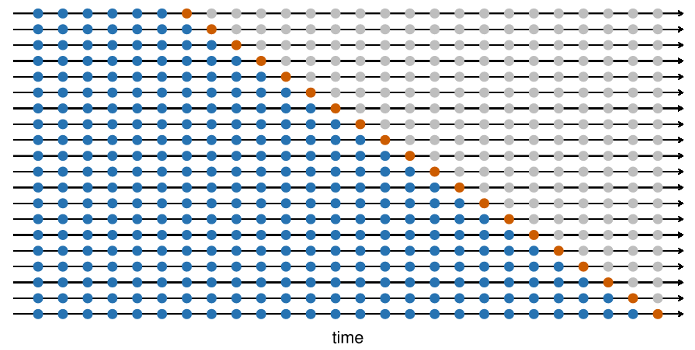
\includegraphics[scale=0.9]{Figure2.png}}

\section{Robustness Check}
With 60\% of the total sample set as in-sample data and the rest as out-of-sample data, the model regressed using the in-sample data is tested outside the sample.

In the multiple linear regression model, the in-sample determinable coefficients are still good, but the out-of-sample determinable coefficients perform poorly, and the fitted curves can also visualize this. The reason for this phenomenon is the over-fitting problem caused by adding too many variables when setting up the model, and fitting the noise in the data into the model. It can also be found that the out-of-sample R-squared is even negative for two-year and three-year bonds, while the out-of-sample prediction improves as maturity rises, which we explain by the fact that the noise cancels each other out as the time period increases.

\begin{table*}[htp!]
    \centering
    \caption{OLS: Result of Robustness Check}
    \setlength{\tabcolsep}{4mm}{
    \begin{threeparttable} 
    \begin{tabular}{ccccc}
        \toprule
            & Panel A    & Panel B    & Panel C    & Panel D     \\
            & $rx^{(2)}$ & $rx^{(3)}$ & $rx^{(4)}$ & $rx^{(5)}$  \\
        \midrule
        $In-Sample-R^2$  & 0.746 & 0.746 & 0.746 & 0.746\\
        $Out-Sample-R^2$ & -0.5070 & -0.328 & 0.135 & 0.180\\
        \bottomrule
    \end{tabular}
    \begin{tablenotes} 
    \footnotesize
    \item \textit{Note:} Out-of-Sample $R^2$ = $1-\frac{\sum_{j=1}^{T} (y_j-\hat{y}_j)^2}{\sum_{j=1}^{T} (y_j-\overline{y}_j)^2}$
    \end{tablenotes} 
    \end{threeparttable} 
    }
\end{table*}

\centerline{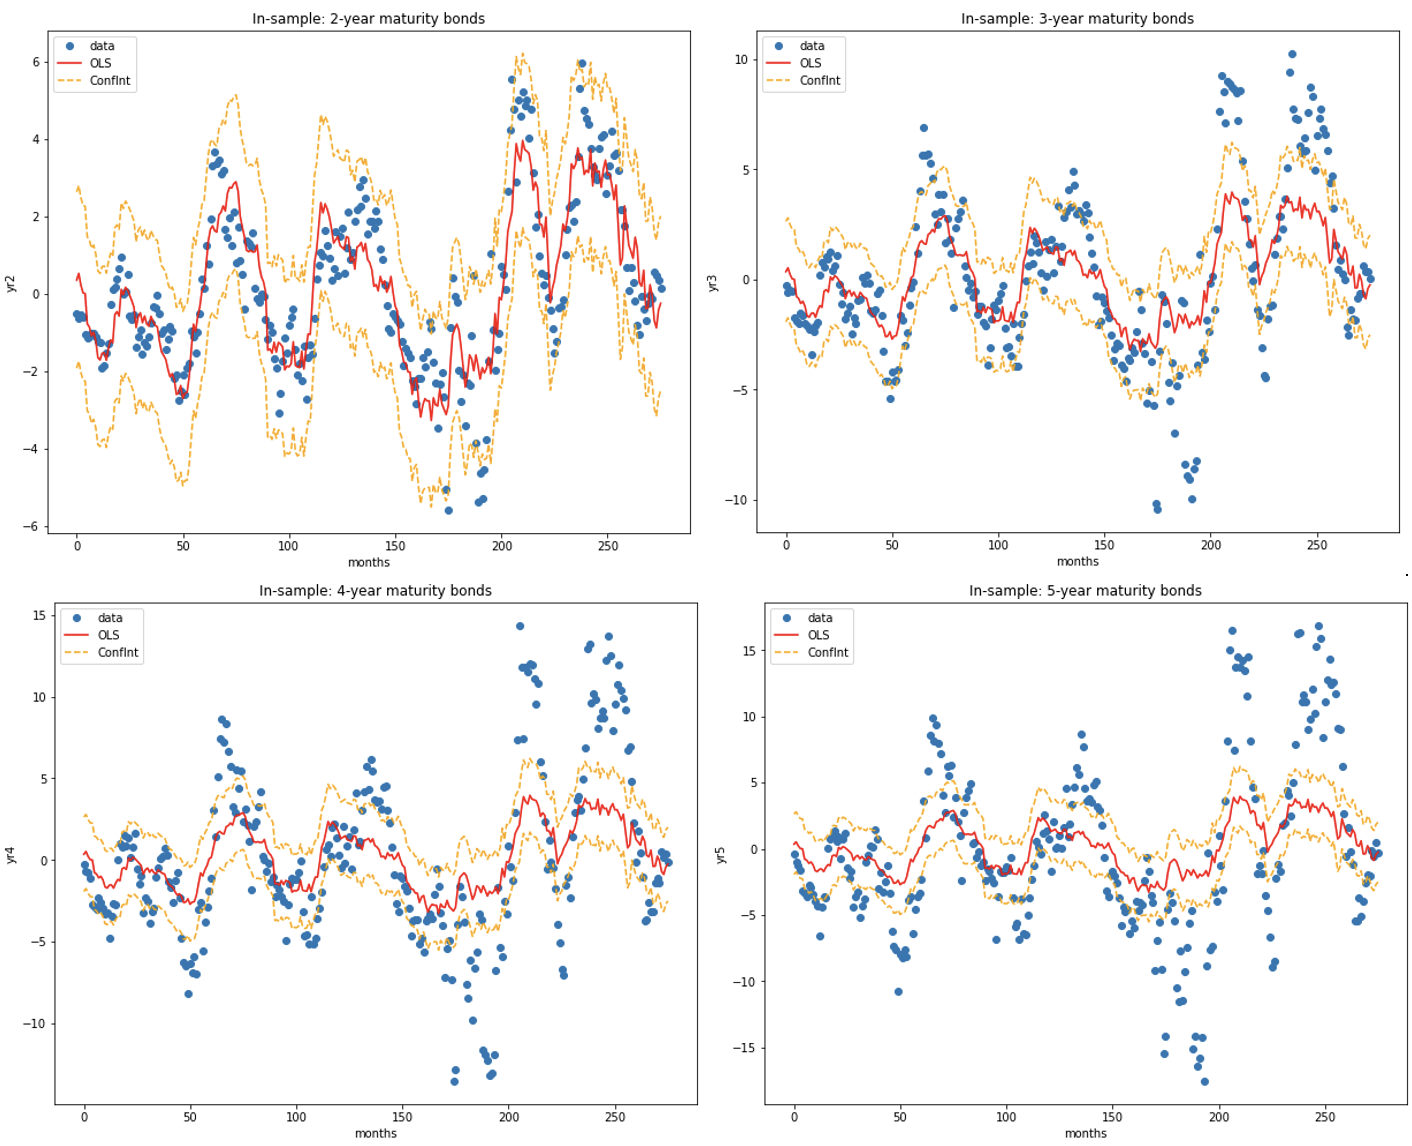
\includegraphics[scale=0.55]{Figure3.png}}
\centerline{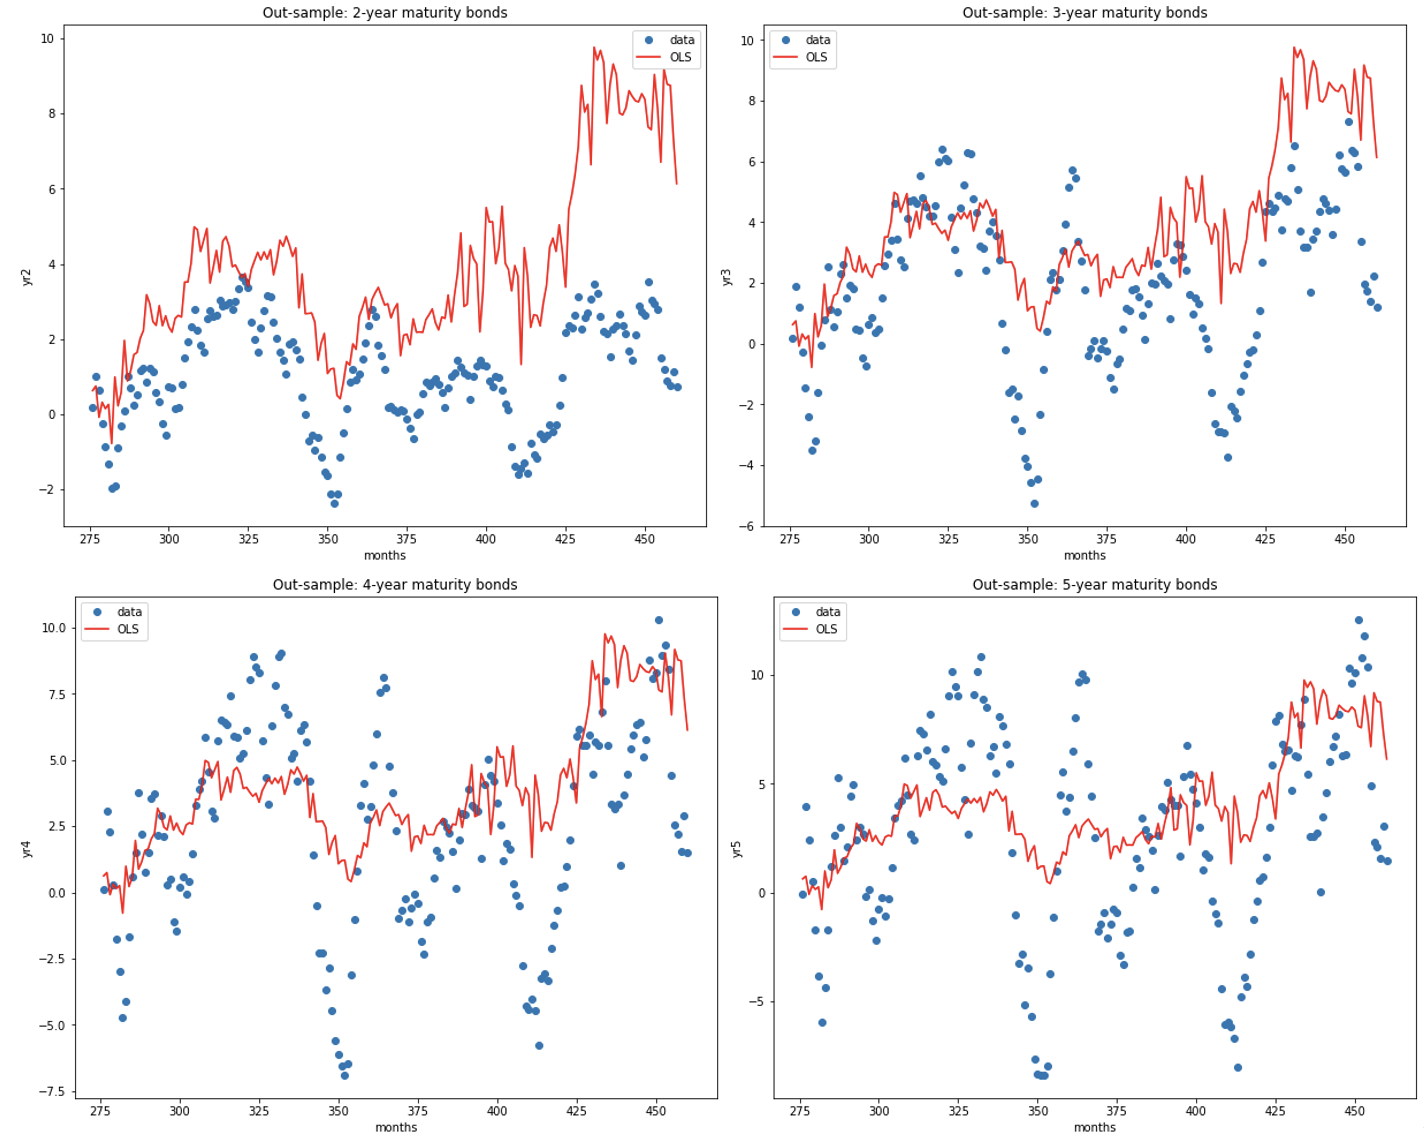
\includegraphics[scale=0.55]{Figure4.png}}
As for machine learning, after cross-validation to adjust the hyperparameters and bringing in out-of-sample data regression, the model achieves good explanatory power in the training group, cross-test group and out-of-sample prediction group. Meanwhile, a simple strategy is constructed, i.e., buying bonds when the excess return is predicted to be positive, otherwise no operation is performed, and the yield is simulated in the out-of-sample data, and positive returns are achieved in all four groups of bonds with different maturities.

\begin{table*}[htp!]
    \centering
    \caption{XGBoost: Result of Robustness Check}
    \setlength{\tabcolsep}{4mm}{
    \begin{threeparttable} 
    \begin{tabular}{ccccc}
        \toprule
            & Panel A    & Panel B    & Panel C    & Panel D     \\
            & $rx^{(2)}$ & $rx^{(3)}$ & $rx^{(4)}$ & $rx^{(5)}$  \\
        \midrule
        TrainingSet, accuracy  & 0.97 & 0.97 & 0.96 & 0.97\\
        TrainingSet, AUC & 1.00 & 1.00 & 0.99 & 0.99\\
        CvSet, accuracy & 0.44 & 0.36 & 0.36 & 0.40\\
        CvSet, AUC & 0.74 & 0.74 & 0.77 & 0.84\\
        OutSample, accuracy & 0.58 & 0.59 & 0.60 & 0.58\\
        OutSample, AUC & 0.85 & 0.82 & 0.80 & 0.78\\
        \bottomrule
    \end{tabular}
    \begin{tablenotes} 
    \footnotesize
    \item \textit{Note:} 
    \item{1} Accuracy, calculated using the ‘$accuracy_score$’ function in sklearn, is the accuracy of the comparison between the predicted label and the real label; 
    \item{2} AUC (Area under the Curve of ROC), calculates the area of the curve ROC, 0.5 < AUC < 1, which is better than random guessing, that is, this classifier (model) can have predictive value if the threshold is properly set.
    \end{tablenotes} 
    \end{threeparttable} 
    }
\end{table*}

\centerline{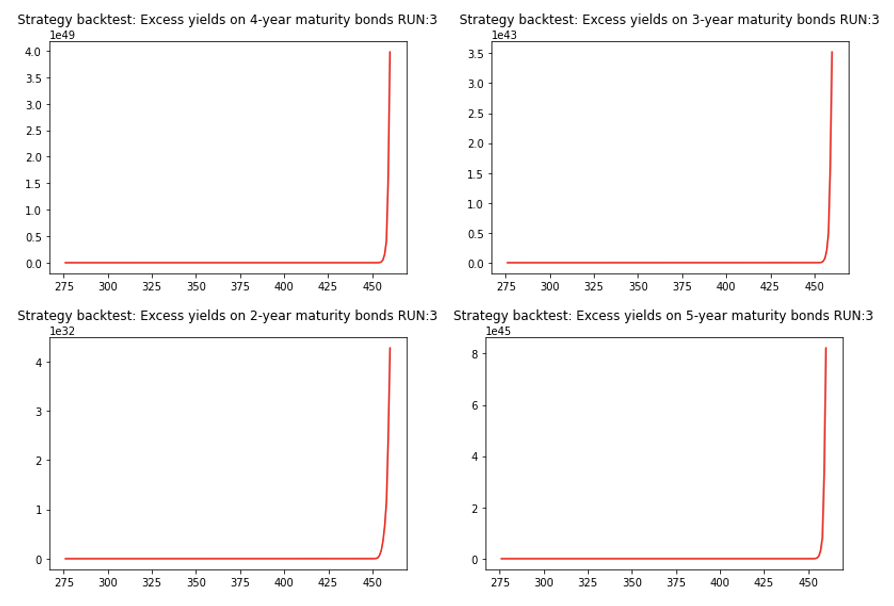
\includegraphics[scale=0.9]{Figure5.png}}

\section{Conclusion}
Our main contribution is the comprehensive analysis through the addition of multiple factors, that is above and beyond the information contained in the term structure of bonds and macroeconomic factors. Also, we back-tested our model with a simple trading strategy and confirmed that it is possible to learn these variables using the XGBoost model to achieve positive returns.

\newpage

\bibliographystyle{unsrt} 
\bibliography{Reference}
\addcontentsline{toc}{section}{Reference}

\newpage

\appendix
\section*{Appendix A. Data Source}
We use some of the data provided by Dr. Xu, and the rest are public datasets from references. Please contact us if you want the full dataset.

\section*{Appendix B. Code}
The code we used could be found at another file, which is named as “The code of group project.ipynb”. Please contact us if you couldn't find it.

\addcontentsline{toc}{section}{Appendices}
\addcontentsline{toc}{subsection}{Appendix A. Data Source}
\addcontentsline{toc}{subsection}{Appendix B. Code}


\end{document}
